%!TEX root = ../thesis.tex

\section{従来手法の概要}
従来手法\cite{okada-si2020}では, 地図を用いたルールベース制御器によるナビゲーションの走行を模倣し, 視覚に基づく経路追従行動を獲得した. 従来手法のシステム概要を\figref{Fig:conv-method}に示す. 学習時, 移動ロボットは\figref{Fig:conv-method}(a)に示すようにLiDARとオドメトリを入力とする地図を用いたルールベース制御器によるナビゲーションで走行する. 同時に, 学習器はカメラ画像とナビゲーションの出力であるロボットの目標角速度をend-to-end学習する. 学習後は, \figref{Fig:conv-method}(b)のようにカメラ画像のみを入力とした学習器の出力により走行する. \par また, 1.1章でも述べたように, 目標経路より離れた位置から経路に戻る学習をすることが経路追従をする上で有効である. そのためには, 経路から一度外れる必要がある. しかし, それでは経路から外れる行動も学習してしまう. そこで, 従来手法では, 学習のデータセットに利用する行動と, 学習時にロボットを制御する行動を別々に扱うことができる. これにより, \figref{Fig:old-method3}に示すように経路から離れた位置から経路に戻る行動を学習することができる. 

\newpage
\begin{figure}[h]
  \begin{minipage}[b]{0.5\linewidth}
    \centering
    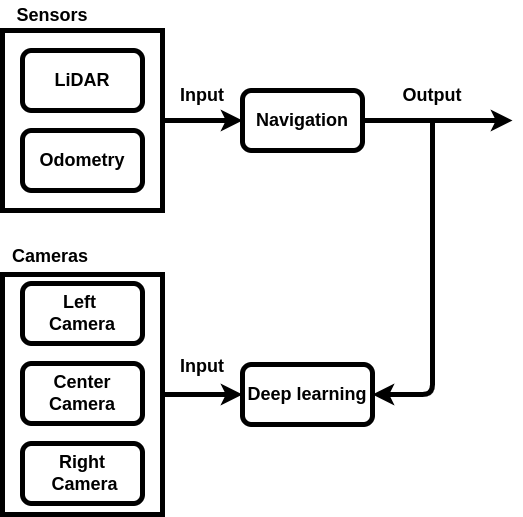
\includegraphics[scale=0.3]{images/old-method1.png}
    \subcaption{Learning phase}
  \end{minipage}
  \begin{minipage}[b]{0.45\linewidth}
    \centering
    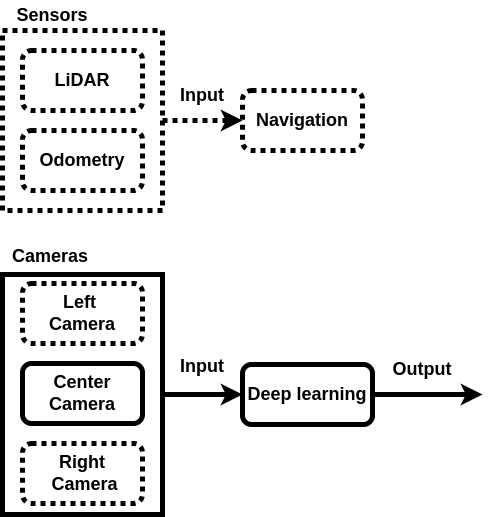
\includegraphics[scale=0.3]{images/old-method2.png}
    \subcaption{Test phase}
  \end{minipage}
  \caption{Conventional method system}
  \label{Fig:conv-method}%\vspace*{-2mm}
\end{figure}

\begin{figure}[h]
  \centering
  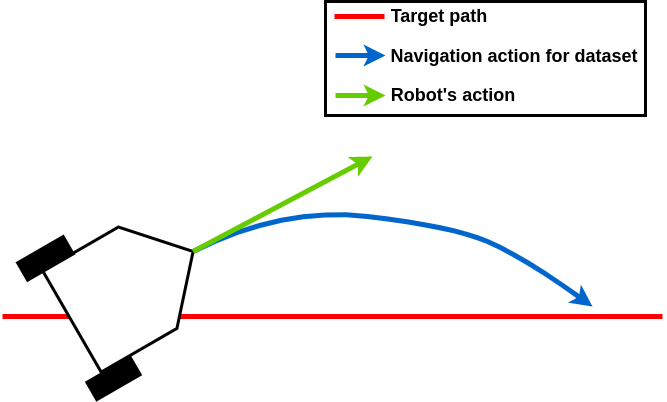
\includegraphics[keepaspectratio, scale=0.4]{images/old-method3.png}
  \caption{The conventional method collects the navigation actions apart from the robot's actions}
  \label{Fig:old-method3}
  \end{figure}

\newpage
\section{従来手法のシステム概要}

